\chapter{Проектная часть}

\section{Описание моделей} \label{section:models}

Для экспериментов были реализованы следующие модели:
\begin{itemize}
\item оконная (WindowNet) - данная модель подробно описана в разделе \ref{subsubsection:window},
\item сверточная (ConvNet) - данная модель подробно описана в разделе \ref{subsubsection:conv},
\item полносвязная нейронная сеть для работы с разреженными синтактико-семантическими признаками (ComprenoNet),
\item комбинация сверточной и полносвязной сети (ConvNet + ComprenoNet)
\end{itemize}

\subsection{Гиперпараметры моделей и признаки}

Общие для всех моделей гиперпараметры:
\begin{itemize}
\item $\alpha=0.01$ - шаг обучения,
\item $p=0.5$ - вероятность для Dropout слоя,
\item количество нейронов в последнем полносвязном слое равно 17,
т.к. используется схема IOBES. Четыре для каждого из четырех типов тегов и один для Outside.
\end{itemize}

Гиперпараметры для оконной модели (рис. \ref{figure:window_net}) следующие:
\begin{itemize}
\item $d_2 = 300$ - количество нейронов в полносвязном слое,
\item $K=5$ - величина окна. Если в окне нет слов, то окно дополняется специальным токеном PADDING,
\item $|T_s|=32$ - размер подмножества для пакетного градиентного спуска.
\end{itemize}

Гиперпараметры для сверточной модели (рис. \ref{figure:conv_net}) следующие:
\begin{itemize}
\item $d_2 = 300$ - количество нейронов в сверточном слое,
\item количество нейронов в полносвязном слое также равно 300,
\item $d_{win} = 3$ - величина окна. Если в окне нет слов, то окно дополняется специальным токеном PADDING,
\item $|T_s|=33$ - размер подмножества для пакетного градиентного спуска.
\end{itemize}

Для экспериментов были использованы следующие признаки:
\begin{itemize}
\item Embeddings - векторные представления слов Senna Embeddings,
\item Capitalization - дискретный признак капитализации слова с 5 возможными вариантами
(слово начинается с большой буквы, слово содержит большую букву,
все символы в слове состоят из больших букв, нет больших букв в слове, не слово),
\item Position - кодирование позиции слова в предложении (описано в разделе \ref{subsubsection:conv}),
\item Gazetteer - проверяется присутствие слова в газетире CoNLL 2003,
\item Compreno sparse features - синтактико-се\-ман\-ти\-ческие признаки Compreno размерности 83951,
\item Compreno SVD 1024 - синтактико-семантически признаки Compreno размерности 83951 были сжаты с использованием
модификации сингулярного разложения для работы с разреженными признаками
TruncatedSVD\footnote{http://scikit-learn.org/stable/modules/generated/sklearn.decomposition.TruncatedSVD.html}
до размерности 1024. После сжатия описываемая дисперсия была равна 72\%. Т.е. потерялось 28\% информации.
\end{itemize}

Все признаки, кроме Compreno sparse features, были включены в нейронные сети с использованием Lookup Table.


\subsection{ComprenoNet}

Архитектура и гиперпараметры полносвязной нейронной сети для работы с разреженными
синтактико-семантическими признаками (ComprenoNet) представлены ниже:
\begin{lstlisting}
input -> (1) -> (2) -> (3) -> (4) -> (5) -> (6) -> (7) -> output
(1): nn.SparseLinear(83951, 256)
(2): nn.Dropout(0.5)
(3): nn.HardTanh
(4): nn.Linear(256 -> 256)
(5): nn.Dropout(0.5)
(6): nn.HardTanh
(7): nn.Linear(256 -> 17)
\end{lstlisting}

SparseLinear представляет из себя обычный полносвязный слой (Linear), который
оптимизирован для работы с разреженными данными. Другие слои и процесс обучения
аналогичны тем, что были описаны в разделе \ref{subsection:nn}.
Общий алгоритм работы сети следующий:
\begin{enumerate}
  \item на вход подается разреженный вектор признаков слова (размерность 83951) для которого предсказывается тег.
  \item Далее этот вектор пропускается через 2 полносвязных слоя.
  \item На выходе еще один полносвязный слой, который выдает вероятность определенного тега.
  Выходов также 17.
\end{enumerate}

\subsection{ConvNet + ComprenoNet}

Архитектура и гиперпараметры комбинации сверточной и полносвязной сети (ConvNet + ComprenoNet)
представлены на рис. \ref{figure:two_net}.
\begin{figure}[!h]
  \centering
  \caption{Комбинация сверточной и полносвязной сети (ConvNet + ComprenoNet)}
  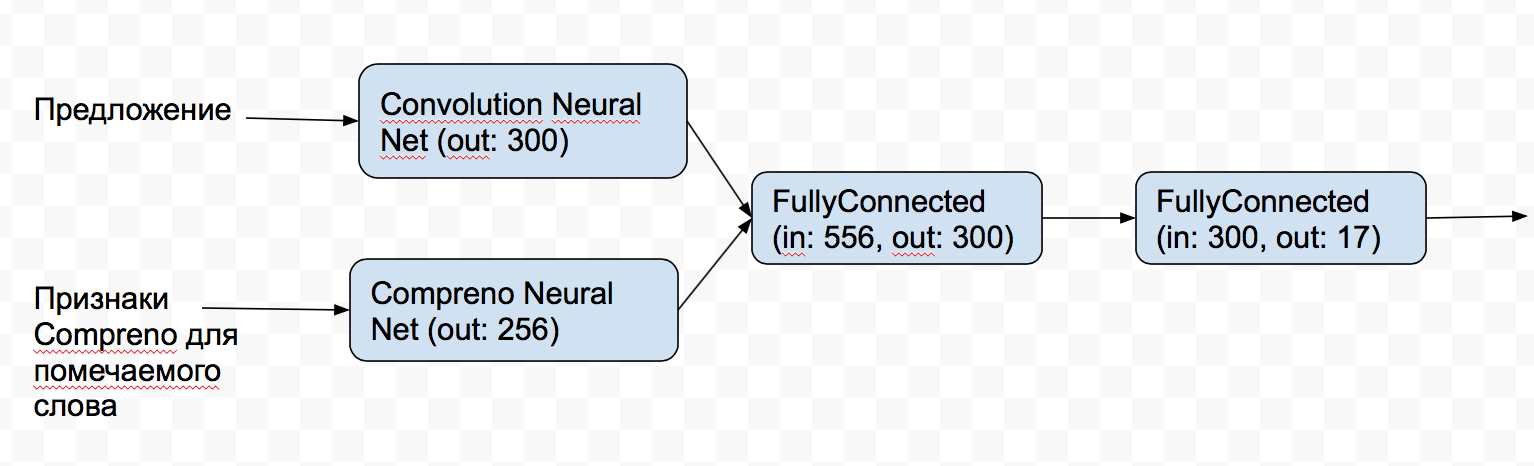
\includegraphics[scale=0.5]{figures/two-net.png}
  \label{figure:two_net}
\end{figure}
Эти сети соединяются следующим образом:
\begin{enumerate}
  \item Из обеих нейросетей удаляются выходные слои.
  \item Предыдущие слои из обеих сетей соединяются в новый полносвязный слой.
  \item Новый полносвязный слой соединяется с выходным слоем. Выходов как и тегов 17.
\end{enumerate}
Веса у объединенной сети были инициализированы предобученными моделями (ConvNet, ComprenoNet).
Слои нейронной сети и процесс обучения аналогичны тем, что были описаны в разделе \ref{subsection:nn}.

\section{Программная реализация}

Для программной реализации описанных выше моделей существуют различные фреймворки
для нейронных сетей.
\textit{Фреймворк}, согласно Википедии\footnote{\url{https://en.wikipedia.org/wiki/Software_framework}} - это
программная платформа, определяющая структуру программной системы; программное обеспечение,
облегчающее разработку и объединение разных компонентов большого программного проекта.

Выбору фреймворка для работы с нейросетями посвящена работа \citep{bahrampour2015comparative}.
В ней они сравнивали такие программные платформы как:
\begin{itemize}
\item Caffe,
\item Neon,
\item TensorFlow,
\item Theano,
\item Torch.
\end{itemize}
В таблице \ref{table:framework_comparison} из \citep{bahrampour2015comparative}
указаны особенности этих фреймворков.

\begin{table}[!h]
  \caption{Особенности нейросетевых фреймворков}
  \centering
  \begin{tabulary}{\textwidth}{| L | L | L | L | L | L | L |}
    \hline\hline
    \multicolumn{1}{|p{1.7cm}|}{Фреймворк} & Caffe & Neon & TensorFlow & Theano & Torch \\
    \hline
    Язык & C++ & Python & C++ & Python & Lua \\
    \hline
    CPU & + & + & + & + & + \\
    \hline
    Поддержка многопоточ-и CPU & + & - & + & + & + \\
    \hline
    GPU & + & + & + & + & + \\
    \hline
    Поддержка неск-х GPU & + & + & + & - & + \\
    \hline
    Nvidia cuDNN & + & - & + & + & + \\
    \hline
    Простота модификации & - & - & +- & + & + \\
    \hline
    Поддержка сообществом & +++ & + & ++ & +++ & ++ \\
    \hline
  \end{tabulary}
  \label{table:framework_comparison}
\end{table}

Практически все современные нейросетевые библиотеки поддерживают работу
с графическими процессорами (GPU).
Производители GPU делают специальные библиотеки для научных
вычислений на графических процессорах.
Например, Nvidia cuDNN (NVIDIA CUDA Deep Neural Network library) -
библиотека, которая ускоряет вычисления для нейронных сетей.
Использование графических процессоров позволяет ускорить обучение нейросетей
в разы по сравнению с центральным процессорным устройством (CPU).
Некоторые фреймворки поддерживают работу с несколькими GPU одновременно для
еще более быстрой работы нейросетей.

Есть программные платформы заточенные для решения одной определенной задачи.
Например, Caffe - нейросетевой фреймворк для решения задач связанных с компьютерным зрением.
Его использование для текстовых данных является затруднительным.
В то же время есть универсальные фреймворки, такие как Torch, TensorFlow,
которые позволяют решать задачи с использование нейронных сетей в различных
областях, включая автоматическую обработку текстов.
Они имеют гибкую архитектуру, поэтому их можно достаточно просто модифицировать.

Все фреймворки описанные в таблице \ref{table:framework_comparison} являются
общедоступными, имеют открытый код и поддерживаются сообществом разработчиков и
разными компаниями. Например, TensorFlow поддерживает компания Google, torch
компания Facebook.

Также стоит отметить, что сверточная модель описанная в разделе \ref{subsubsection:conv}
уже имеет программную реализацию в открытом доступе в сети по адресу: http://ronan.collobert.com/senna/.
Минусом данной реализации является то, что она написана без использования
нейросетевых фреймворков, на языке программирования C, не поддерживает GPU,
не поддерживается сообществом, имеет тяжелый в понимании код, заточена под конкретную задачу
и не содержит в себе различные современные нейросетевые решения, например Dropout.

Исходя из следующих требований:
\begin{itemize}
\item гибкость в реализации нейросетевых архитектур,
\item быстрота проведения экспериментов,
\item поддерживаемый код,
\end{itemize}
был выбран нейросетевей фреймворк torch\footnote{\url{http://torch.ch}}.

Код для воспроизведения экспериментов выложен по адресу:
\href{https://github.com/sld/torch-conv-ner}{github.com/sld/torch-conv-ner}.

Скорость обучения на машине с GPU Amazon AWS g2.2xlarge\footnote{https://aws.amazon.com/ru/ec2/instance-types/}:
\begin{itemize}
\item 1 эпоха\footnote{Эпоха - это один полный проход по обучающей выборке} при одиночной обработке (stochastic gradient descent): $\sim$450 сек.
\item 1 эпоха при пакетной обработке (mini-batch gradient descent): $\sim$171 сек.
\item Модель получающая 87.49\% обучалась 91 эпоху ($\sim$4.2 часа).
\item 1 эпоха при пакетной обработке с использованием признаков Compreno: $\sim$615 сек.
\end{itemize}

Скорость классификации составляет 2500 токенов в секунду при пакетной обработке.

\newpage

\section{Эксперименты}

\subsection{Эксперименты без синтактико-семантических признаков}
По таблице \ref{table:raw_net} видно, что результаты немного ниже чем у \citep{collobert2011natural}.
Это связано с тем, что для Window подхода использован другой метод оптимизации,
а для Convolution подхода не были применены условные случайные поля (ConvNet + CRF в таблице \ref{table:raw_net}).

В качестве референсной, будет использована модель из последнего эксперимента
показывающая 87.49\% F1.
Это сделано для чистоты эксперимента, т.к. далее  обучение происходило только
на обучающей выборке по правилам соревнования CoNLL 2003 и применялся пакетный
градиентный спуск для ускорения экспериментов.

\newpage

\begin{table}[!h]
  \caption{Результаты экспериментов без использования синтактико-семантических признаков}
  \centering
  \begin{tabulary}{\textwidth}{| L | L | L | L | L | L |}
    \hline\hline
    \multicolumn{1}{|p{1.7cm}|}{Модель} & Признаки & Выборка & Метод оптимизации & Полученная F1, \% & F1 в статье \cite{collobert2011natural} \\
    \hline
    Window & Embeddings, Capitalization & train & Mini-batch gradient descent & 86.27 & - \\
    \hline
    Window & Embeddings, Capitalization & train & Stochastic gradient descent & - & 86.97 \\
    \hline
    ConvNet + CRF & Embeddings, Capitalization, Position & train & Stochastic gradient descent & - & 88.67 \\
    \hline
    ConvNet + CRF & Embeddings, Capitalization, Position, Gazetteer & train & Stochastic gradient descent & - & 89.59 \\
    \hline
    ConvNet & Embeddings, Capitalization, Position & train & Stochastic gradient descent & 86.77 & - \\
    \hline
    ConvNet & Embeddings, Capitalization, Position, Gazetteer & train & Stochastic gradient descent & 87.89 & - \\
    \hline
    ConvNet & Embeddings, Capitalization, Position, Gazetteer & train + dev & Stochastic gradient descent & 88.37 & - \\
    \hline
    ConvNet & Embeddings, Capitalization, Position, Gazetteer & train & Mini-batch gradient descent & \textbf{87.49} & - \\
    \hline
  \end{tabulary}
  \label{table:raw_net}
\end{table}

\subsection{Эксперименты с синтактико-семантическими признаками сжатыми с использованием SVD}

\begin{table}[!h]
  \caption{Результаты с синтактико-семантическими признаками сжатыми SVD}
  \centering
  \begin{tabulary}{\textwidth}{| L | L | L | L | L | L |}
    \hline\hline
    \multicolumn{1}{|p{1.7cm}|}{Модель} & Признаки & Выборка & Метод оптимизации & Полученная F1, \% \\
    \hline
    ConvNet & Position, Compreno SVD 1024 & train & Mini-batch gradient descent & 75.89 \\
    \hline
    ConvNet & Capitalization, Position, Gazetteer, Compreno SVD 1024 & train & Mini-batch gradient descent & 81.83 \\
    \hline
    ConvNet & Embeddings, Capitalization, Position, Gazetteer, Compreno SVD 1024 & train & Mini-batch gradient descent & 86.85 \\
    \hline
    ConvNet & Embeddings, Capitalization, Position, Gazetteer & train & Mini-batch gradient descent & 87.49 \\
    \hline
  \end{tabulary}
  \label{table:svd_net}
\end{table}


По таблице \ref{table:svd_net} видно, что такой способ ведет к небольшому ухудшению F1-меры.
Это может быть связно с тем, что после применения сингулярного разложения
было потеряно 28\% информации о синтактико-семантических признаках Compreno.


\subsection{Эксперименты с синтактико-семантическими признаками на ConvNet + ComprenoNet}

Веса у ConvNet + Compreno Net были инициализированы обученными моделями -
моделью показывающую 87.49\% для сверточной сети и моделью показывающую
72.85\% (см. таблицу \ref{table:union_net}) для второй нейронной сети.

\begin{table}[ht]
  \caption{Результаты с синтактико-семантическими признаками для объединенной нейросети}
  \centering
  \begin{tabulary}{\textwidth}{| L | L | L | L | L | L |}
    \hline\hline
    \multicolumn{1}{|p{1.5cm}|}{Модель} & Признаки & Выборка & Метод оптимизации & Полученная F1, \% \\
    \hline
    Compreno Net & Compreno sparse features & train & Mini-batch gradient descent & 72.85 \\
    \hline
    ConvNet & Embeddings, Capitalization, Position, Gazetteer & train & Mini-batch gradient descent & 87.49 \\
    \hline
    ConvNet + Compreno Net & Embeddings, Capitalization, Position, Gazetteer, Compreno sparse features & train & Mini-batch gradient descent & \textbf{88.47} \\
    \hline
    ConvNet + Compreno Net & Embeddings, Capitalization, Position, Gazetteer, Compreno sparse features & train + dev & Mini-batch gradient descent & 88.81 \\
    \hline
  \end{tabulary}
  \label{table:union_net}
\end{table}

По таблице \ref{table:union_net} видно, что в этом случае признаки Compreno
улучшают F1-меру почти на один процент.
